%%
%% Author: samuelblattner
%% 2019-01-20
%%

% Preamble
\documentclass{ffhsthesis}

% Packages
\usepackage{amsmath}
\usepackage[utf8]{inputenc}
\usepackage[bibstyle=apa,backend=biber]{biblatex}

% Listings
\usepackage{listings}
\usepackage{color}

\definecolor{codegreen}{rgb}{0,0.6,0}
\definecolor{codegray}{rgb}{0.5,0.5,0.5}
\definecolor{codepurple}{rgb}{0.58,0,0.82}
\definecolor{backcolour}{rgb}{0.95,0.95,0.92}

\lstdefinestyle{mystyle}{
backgroundcolor=\color{backcolour},
commentstyle=\color{codegreen},
keywordstyle=\color{magenta},
numberstyle=\tiny\color{codegray},
stringstyle=\color{codepurple},
basicstyle=\footnotesize,
breakatwhitespace=false,
breaklines=true,
captionpos=b,
keepspaces=true,
numbers=left,
numbersep=5pt,
showspaces=false,
showstringspaces=false,
showtabs=false,
tabsize=2
}

\lstset{style=mystyle}
\addbibresource{sema-samuel-blattner.bib}
\usepackage[hidelinks]{hyperref}
\usepackage{glossaries}

\makeglossaries

\newglossaryentry{neuron}
{
name=Neuron,
plural=Neuronen,
description="Ein Neuron ist ein…"
}

\newglossaryentry{Tokenizer}
{
name=Tokenizer,
plural=Tokenizers,
description="Ein Tokenizer ist ein..."
}
\makeglossaries
\makeglossary

% Document
\begin{document}

    \dokumentTyp{Bachelor/Master-Thesis}
    \studiengang{INF/WI}
    \title{Recurrent Neuronal Networks als Kreativitätswerkzeug für Gastronomiebetriebe}
    \titelbild[height=2cm,width=10cm]{ffhslogo}  % optional
    \author{Samuel Blattner}
    \wohnort{Zürich}

    \referentin{Dr. Heinrich Zimmermann\\ BSc INF 2015, ZH5-Mo, FS19}
    \eingereichtBei{Dr. Heinrich Zimmermann\\ BSc INF 2015, ZH5-Mo, FS19}

    \maketitle

    \begin{zusammenfassung}

    \end{zusammenfassung}

    \begin{abstract}
        ... English summary ...
    \end{abstract}

    \setcounter{tocdepth}{1}
    \tableofcontents

    \startThesis % Befehl muss vor dem ersten chapter stehen (Seitennummerierung!)

    \chapter{Einleitung}
\label{ch:introduction}

Die Gastronomie hat sich im vergangenen Jahrzehnt nach eigener Wahrnehmung des Autors zu einem äusserst populären Thema entwickelt.
Haupttreiber dafür sind sicherlich Social Media, auf denen kreative Lokale, ausgefallene Gerichte und besondere Momente weltweit geteilt werden.
Andererseits tragen auch ein neues Ernährungsbewusstsein, die weltweite Mobilität sowie Berichterstattungen über Gastronomiebetriebe, beispielsweise als TV-Serie, zum wachsenden Interesse bei.
Der Markt ist hart umkämpft, und Restaurants kommen und gehen insbesondere in Stadtgebieten in hohen Raten, wie eine neuere Statistik der Stadt Zürich zeigt\footnote{https://www.zkb.ch/media/pub/coporate/zuerich-in-zahlen/kt-zh-zahlen-223653.pdf}.
Der gesättigte Markt zwingt die Betriebe zu Effizienz, Innovation und zu möglichst hoher Qualität.
Unlängst hat deshalb auch die Digitalisierung in Gastronomiebetrieben Einzug gehalten, werden doch zumindest Reservationen immer häufiger online getätigt\footnote{https://www.lunchgate.info/blog/gastronomie-digitalisierung}, Bestellungen via Tablet
direkt in die Küche gesendet und Rechnungen per App unter Freunden aufgeteilt.
All diese Entwicklungen beschäftigen sich primär mit der Automatisierung von Prozessen.
Wie aber können Gastronomiebetriebe in anderen Bereichen, wie z.B. der Kreativität unterstützt werden?
Diese Arbeit geht folgender Frage nach: «Kann ein neuronales Netz durch Training mit einfachen Namen von Gerichten sinnvolle, neue und parameterabhängige Namen erzeugen?»
Diese Arbeit untersucht, ob und wie ein Neuronales Netz als Kreativitätswerkzeug bzw. Namensgenerator für Speisen verwendet werden kann.

    \chapter{Modell}
\label{ch:model}

Dieser Teil beschreibt das der Arbeit zugrunde liegende Modell.
Das Modell wird hierbei in seiner finalen Ausführung dargestellt.
Dieser liegen diverse Iterationen von Experimenten und Verbesserungen zugrunde, die jedoch für das Verständnis des
Modells keine Relevanz haben und auf die nicht weiter eingegangen wird.
Einzig die Behebung eines Implementierungsfehlers sowie die damit verbundene Änderung in der Art und Weise, wie das Modell trainiert wird,
sollen kurz beleuchtet werden, da sie für den Leser wertvolle Hinweise für eigene Implementierungen bieten können.

\section{Daten \& Training}
\label{sec:model-data-training}

In diesem Abschnitt werden die Trainingsdaten für das Modell analysiert und beschrieben.
Als Lerngrundlage für den Algorithmus dienen rund 400000 Namen von Gerichten.
Diese sind im Kaggle-Datensatz «What's on the menu»\footnote{https://www.kaggle.com/nypl/whats-on-the-menu}\footnote{http://nypl.github.io/menus-api/} enthalten.
Der Unterdatensatz «Dish.csv» enthält folgende Struktur:


\begin{center}
    \resizebox{\textwidth}{!}{
    \begin{tabular}{ |r|l|r|r|r|r|r|r| }
        \hline
        \textbf{id} & \textbf{name} & \textbf{menus\_appeared} & \textbf{times\_appeared} & \textbf{first\_appeared} & \textbf{last\_appeared} & \textbf{lowest\_price} & \textbf{highest\_price} \\
        \hline
        1 & Consomme printaniere royal  &    8 &    9 & 1897 & 1927 & 0.2  & 0.4 \\
        \hline
        2 & Chicken gumbo               &  110 &  116 & 1895 & 1960 & 0.1  & 0.8 \\
        \hline
        3 & Tomato aux croutons         &   13 &   13 & 1893 & 1917 & 0.25 & 0.4 \\
        \hline
        4 & Onion au gratin             &   41 &   41 & 1900 & 1971 & 0.25 & 1   \\
        \hline
        5 & Radishes                    & 3265 & 3349 & 1854 & 2928 & 0    & 25  \\
        \hline
        6 & Chicken soup with rice      &   48 &   49 & 1897 & 1961 & 0.1  & 0.6 \\
        \hline
        … & … & … & … & … & … & … & … \\
        \hline
    \end{tabular}
    }
\end{center}

Für die Arbeit relevant ist vorerst lediglich die \textit{name}-Spalte.
Sie enthält Bezeichungen von Gerichten in mehreren Sprachen.

Für das Training eines ersten Modells wird folgende Spezifikation verwendet:

Batches: 100
Batchsize: 50
Epochen: 50
RNN-Units: 64
RNN-Layers: 1
Textlänge: 15

Für die Validierung pro Epoche werden jeweils die weiteren Zeilen, die auf das Trainingsset folgen, verwendet.



\section{Formale Definition}
\label{sec:model-definition}

Weil sie fähig sind, zeitliche Zustände zu speichern, eignen sich Rekurrente Neuronale Netze (in der restlichen Arbeit wird die Abkürzung «RNN» verwendet) besonders gut, um Sequenzen zu lernen.
Die natürliche Sprache ist eine Sequenz von Wörtern, die in sich wiederum aus einer Sequenz von Buchstaben bestehen.
Deshalb kommen RNNs bis heute in vielen Gebieten von natürlichsprachlicher Textverarbeitung zum Einsatz.

Die Besonderheit eines RNN's liegt darin, dass – anders als bei einfachen neuronalen Netzen – die \glspl{neuron} nicht nur den Wert der vorangehenden Netzschicht als
Eingangswert erhalten, sondern auch den Ausgangswert des vorangehenden Zeitschritts ihrer selbst.
Jedes \gls{neuron} speichert den Zustand der bisherigen Zeitschritte als sog. «hidden state», der mit der Variable $ h $ gekennzeichnet wird (siehe Abb. \ref{fig:rnn-model-definition}).
Für nähere Details zur Architektur und Funktionsweise sei auf die exzellente Beschreibung in \autocite{geron} verwiesen.

\begin{figure}
    \centering
    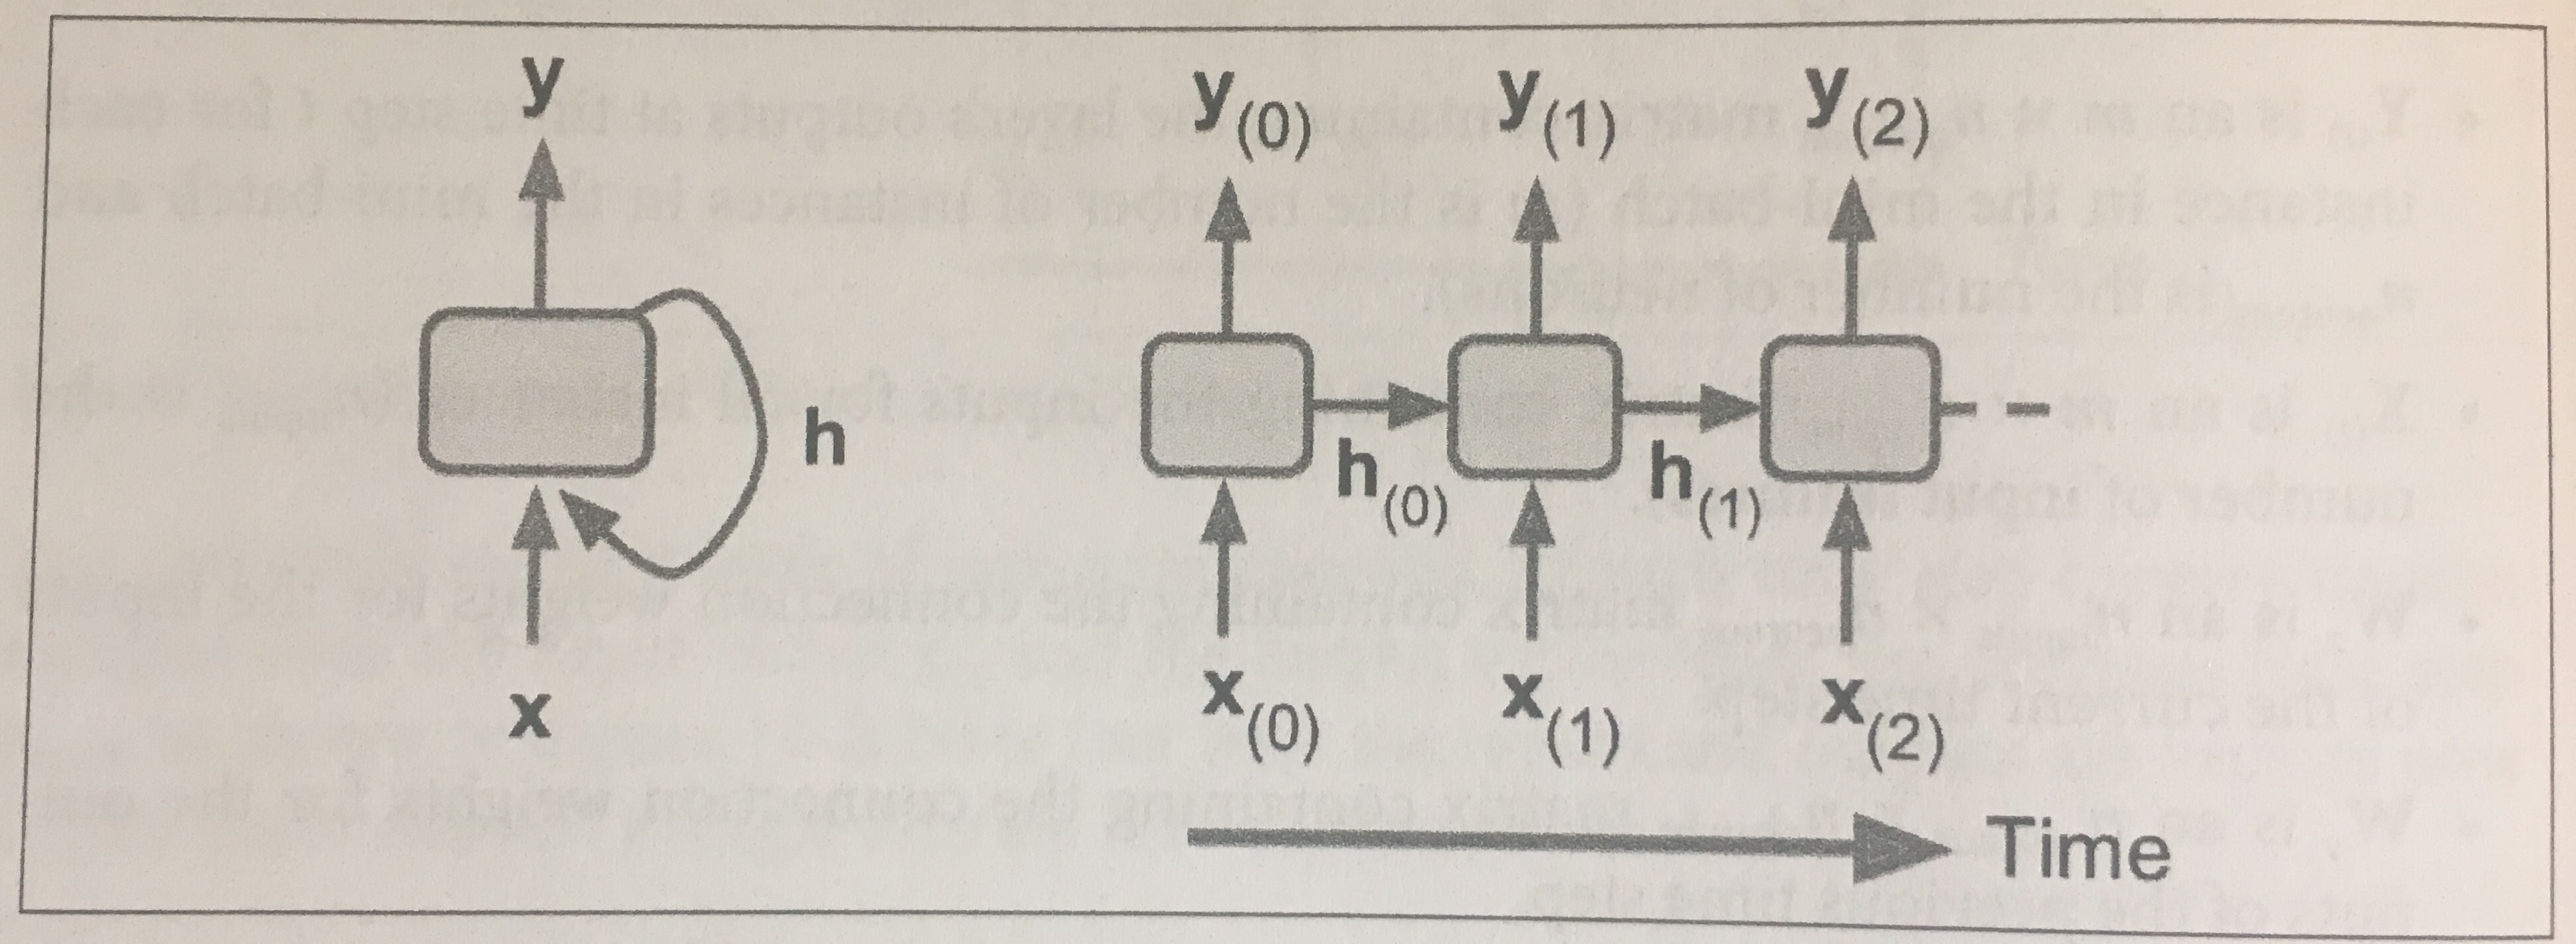
\includegraphics[width=0.75\linewidth]{images/model/model-rnn-definition.jpg}
    \caption[RNN Modell]{RNN Modell \autocite{geron}}
    \label{fig:rnn-model-definition}
\end{figure}

Zwei gut bekannte Probleme, die einfache RNN-Memory-Zellen aufweisen sind einerseits das sog. «Exploding/Vanishing Gradient Problem», bei dem insbesondere in mehrschichtigen neuronalen Netzen
die propagierten Werte «explodieren» oder gegen null «verschwinden», andererseits das Problem, dass anfangs eingespeiste Informationen gegen Ende der Sequenz verloren gehen \autocite{geron}.
Zur Lösung dieser Problem wurden sog. «Long-Short-Term Memory Cells» (LSTM)\autocite{lstm} und später sog. «Gated Recurrent Units» (GRU)\autocite{gru} entwickelt.
Weil sich beide «Gedächtniszellen» als sehr erfolgreich bewiesen haben, werden einfache RNN-Zellen schon fast nicht mehr verwendet.


\section{Implementierung}
\label{sec:model-implementation}

Für den Aufbau und das Training werden TensorFlow 2.0\footnote{https://www.tensorflow.org/beta} sowie das mittlerweile darin integrierte Framework Keras\footnote{https://keras.io/} verwendet.
Der Code ist auf Github\footnote{https://github.com/samuelblattner/ffhs-sema} frei verfügbar.
Die Implementierung kann grundsätzlich in drei Komponenten aufteilt werden:

\paragraph{Builder (build.py)} Die Builder-Komponente übernimmt die Aufgabe, das RNN-Modell mit Keras nach bestimmten Vorgaben aufzubauen (z.B. Anzahl LSTM-Einheiten, Anzahl Schichten, …).
Weil Neuronale Netze auf arithmetischen Operationen beruhen, müssen die Eingabezeichen in Zahlen umgewandelt werden.
Diese Aufgabe übernimmt ein sog. «\glq{Tokenizer}».
Die Komponente gibt als Rückgabewert einersets das kompilierte Modell sowie andererseits einen Tokenizer zurück, der numerische Repräsentationen für sämtliche im Datensatz enthaltenen Zeichen (=Vokabular) enthält.

\paragraph{Loader} Der Loader übernimmt die Aufgabe, die Trainings- wie auch Validierungsdaten bereitszustellen.
Das Training des Modells wird im sog. Mini-Batch-Verfahren vollführt.
Der Loader lädt damit mit einem Python-Generator für jede Trainingsepoche nacheinander mehrere Ausschnitte des Gesamtdatensatzes (siehe Listing \ref{lst:mini-batch-loader}, Zeile 3).
Dies ermöglicht, beliebig grosse Datensätze zu bearbeiten, da immer nur der Speicherbedarf eines Mini-Batches benötigt wird.
Der Loader implementiert zudem ein Offset (Zeile 13), mit dem der Datensatz «vorgespult» werden kann.
Damit ist es möglich, vom gleichen Datensatz sowohl das Trainingsset wie auch das Validierungsset zu entnehmen.
Statt vom Anfang des Datensatzes, startet das Validierungsset jedoch viel weiter hinten im Datensatz, im Idealfall – und bei genügend grossem Datensatz – ausserhalb des Bereichs, den das Trainingsset jemals erreichen wird.

\begin{lstlisting}[language=Python, caption=Mini-Batch Loader, label=lst:mini-batch-loader]
    ...
    # Load mini-batch
    for dataframe in read_csv(
        filepath_or_buffer='data.csv',
        delimiter=',',
        header=0,
        chunksize=1000):

        # Iterate over lines in mini-batch
        for row in dataframe[dataframe.columns[1]]:
            ...

            if self.__offset > 0 and offset_lines_skipped < self.__offset:
                offset_lines_skipped += 1
                continue
                ...
\end{lstlisting}

Der Loader übernimmt zudem die Aufgabe, die Textsequenzen in einzelne Trainingseinheiten zu zerlegen.
Eine Trainingseinheit besteht immer aus einer konstanten Anzahl Zeichen (Fenstergrösse) und einem Zielzeichen.
Zudem wird am Schluss eine Stoppmarke («<end>») angefügt, die dem Modell das Ende der Sequenz signalisiert.
Ist eine Trainingssequenz kürzer als die Fenstergrösse, wird sie mit Platzhalter Zeichen aufgefüllt («padding»).
Ist eine Trainingssequenz länger als die Fenstergrösse, so wird sie abgeschnitten.
und Zeichen um Zeichen in mehreren Trainingsschritten durch das Fenster geschoben (siehe Tabelle \ref{tab:splitting-into-training-units}).
Der letzte Buchstabe wird jeweils als Zielwert abgeschnitten und in einem separaten Array zurückgeliefert (y-Wert).
Gleichzeitig werden die Buchstabensequenzen mit dem zuvor erwähnten Tokenizer in Vokabular-Indizes umgewandelt.
Da die Ausgabe des Modells eine Wahrscheinlichkeitsverteilung für alle Buchstaben in Form eines Vektors sein wird (Wertebereich 0.0 - 1.0), ist es
für ein optimales Training erforderlich, auch die Eingabe ins Modell entsprechend umzuformen.
Die Vokabular-Indizes werden umgewandelt in sog. «One-Hot-Vektoren».
Ein One-Hot-Vektor besteht aus sovielen Komponenten, wie das Vokabular Zeichen enthält.
Die Komponenten mit dem Index des entsprechenden Zeichens wird auf $ 1.0 $ gesetzt, alle anderen Komponenten bleiben $ 0.0 $.
Der Eingabevektor ist somit gewissermassen ebenfalls eine Wahrscheinlichkeitsverteilung, allerdings hat genau ein Zeichen die Wahrscheinlichkeit $ 100\% $ (das nächste Zeichen in der Sequenz), während
alle anderen Zeichen die Wahrscheinlichkeit $0.0\%$ haben.
Hat das nächste Zeichen «B», das ins Modell eingegeben werden soll, den Tokenizer-Index 2 (bei einer Vokabulargrösse von insgesamt 5 Zeichen), so würde daraus der One-Hot-Vektor $ (0.0, 0.0, 1.0, 0.0, 0.0, 0.0)^{T} $ gebildet.
Listing \ref{lst:one-hot-encoding} zeigt, wie die Konvertierungsschritte von Zeichen bis One-Hot-Vektor mit den von Keras bereitsgestellten Utility-Funktionen einfach erledigt werden können.

\begin{table}
    \centering
    \footnotesize
    \begin{tabularx}{0.75\textwidth}{|>{\hsize=.1\hsize}X|>{\hsize=.1\hsize}X|>{\hsize=.1\hsize}X|>{\hsize=.1\hsize}X|>{\hsize=.1\hsize}X|>{\hsize=.1\hsize}X|>{\hsize=.1\hsize}X|>{\hsize=.1\hsize}X|>{\hsize=.1\hsize}X||>{\hsize=.1\hsize}X|}
    \hline
    \textbf{0} & \textbf{1} & \textbf{2} & \textbf{3} & \textbf{4} & \textbf{5} & \textbf{6} & \textbf{7} & \textbf{8} & \textbf{Ziel} \\\hline
            pad & pad & pad & pad & pad & pad & pad & pad & pad & C \\\hline
            pad & pad & pad & pad & pad & pad & pad & pad & C & h \\\hline
            pad & pad & pad & pad & pad & pad & pad & C & h & i \\\hline
            pad & pad & pad & pad & pad & pad & C & h & i & c \\\hline
            pad & pad & pad & pad & pad & C & h & C & c & k \\\hline
            pad & pad & pad & pad & C & h & i & c & k & e \\\hline
            pad & pad & pad & C & h & i & c & k & e & n \\\hline
            pad & pad & C & h & i & c & k & e & n & ' ' \\\hline
            pad & C & h & i & c & k & e & n & ' ' & C \\\hline
            C & h & i & c & k & e & n & ' ' & C & u \\\hline
            h & i & c & k & e & n & ' ' & C & u & r \\\hline
            i & c & k & e & n & ' ' & C & u & r & r \\\hline
            c & k & e & n & ' ' & C & u & r & r & y \\\hline
            k & e & n & ' ' & C & u & r & r & y & <end> \\\hline

    \end{tabularx}
    \caption{Zerlegung in Trainingseinheiten am Beispiel der Fenstergrösse 9 (Stellen 0 - 8).
    Der Begriff «Chicken Curry» wird Zeichen um Zeichen durch das Fenster hindurchgeschoben.
    Jede Zeile entspricht einer Trainingseinheit.
    Das Modell versucht das Zielzeichen in der Spalte «Ziel» anhand der Sequenz in den Stellen 0 bis 8 vorherzusagen.}
    \label{tab:splitting-into-training-units}

\end{table}

\begin{lstlisting}[language=Python, caption=Encodierung von Zeichen bis One-Hot-Vektor, label=lst:one-hot-encoding]
    ...

    # Tokenize sequence characters (e.g. ['pad', 'pad', 'B', 'e', 'e', 'r'] -> [2, 2, 5, 4, 4, 1])
    tokenized_char_phrases_X, tokenized_chars_y = windowed_tokenized_sequences[:, :-1], windowed_tokenized_sequences[:, -1]

    # Convert to 1-hot-vector for input into model
    # (e.g. [2, 2, 5, 4, 4, 1] -> [
    #    [0, 0, 1, 0, 0, 0],
    #    [0, 0, 1, 0, 0, 0],
    #    [0, 0, 0, 0, 0, 1],
    #    [0, 0, 0, 0, 1, 0],
    #    [0, 0, 0, 0, 1, 0],
    #    [0, 1, 0, 0, 0, 0],
    # ])
    one_hot_phrases = to_categorical(padded_phrases_X, num_classes=len(tokenizer.index_word) + 1)
    one_hot_ys = to_categorical(tokenized_chars_y, num_classes=len(tokenizer.index_word) + 1)
    ...
\end{lstlisting}


\paragraph{Tainer (train.py)} Trainer ist die Hauptkomponente, die vom Loader und vom Builder gebrauch macht.
Der Trainer führt das eigentliche Training des Modells durch.
Dem Modell werden zudem sog. Callbacks\footnote{https://keras.io/callbacks/} hinzugefügt, damit das Modell nach
längeren Abschnitten ohne Verbesserung nicht unnötig weiter trainiert werden muss und somit Rechenzeit gespart werden kann.
Ausserdem wird das gesamte Modell und insbesondere seine Gewichte nach jeder Epoche quasi als «Spielstand» gespeichert,
falls sich die Validierungsrichtigkeit («Accuarcy») insgesamt verbessert hat.
So wird vermieden, dass ein Modell nach abgebrochenem Training von vorne trainiert werden muss.

\subsection{Hardware \& Evaluierung der günstigsten Mini-Batch-Grösse}
\label{sec:evaluating-fastest-batchsize}
Für das Training des Modells steht eine nVidia GeForce GTX 980 Grafikkarte zur Verfügung.
Aufgrund der für Matritzenoperationen optimierten Hardware eignen sich Grafikkarten besonders gut für Machine Learning.
Unter verwendung des CUDA-Tookits\footnote{https://developer.nvidia.com/cuda-downloads} sowie des Keras-Frameworks kann
die Grafikkarte annähernd transparent ins Training des Modells einbezogen werden.
Während der ersten Versuche konnte eine variiernde Ausführungsgeschwindigkeit in Abhängigkeit der Mini-Batch-Grösse beobachtet werden.
Mini-Batches werden immer als Ganzes der Grafikkarte übergeben.

Um das Modell möglichst effizient zu trainieren, soll die effizienteste Mini-Batch-Grösse für diese Grafikkarte empirisch eruiert werden.
Dazu werden 10 Epochen mit jeweils 1000 Trainingsschritten vollführt.
Die erfassten Laufzeiten in Tabelle \ref{tab:best-batch-size} zeigen auf, dass das Modell bei einer Mini-Batch-Grösse von 100 Trainingseinheiten
am effizientesten zu arbeiten scheint.
Für sämtliche Modellkonfigurationen soll deshalb die Mini-Batch-Grösse von 100 Trainingseinheiten verwendet werden.

\begin{center}
    \begin{table}
        \centering
        \begin{tabular}{ |l|l| }

            \hline
            \textbf{Mini-Batch-Grösse} & \textbf{Durchschnittliche Dauer in Sekunden (über 10 Epochen)} \\
            \hline
            1 & 14.69 \\
            50 & 4.07 \\
            71 & 4.04 \\
            91 & 3.97 \\
            100 & 3.93 \\
            125 & 3.98 \\
            200 & 5.32 \\
            250 & 6.16 \\
            \hline
        \end{tabular}
        \caption{Ausführungszeiten unter Verwendung verschiedener Mini-Batch-Grössen}
        \label{tab:best-batch-size}
    \end{table}
\end{center}


\subsection{Implementierungsfehler \& Erweiterung des Trainingssets}
\label{subsec:enhancing-training-set}

\begin{figure}
    \centering
    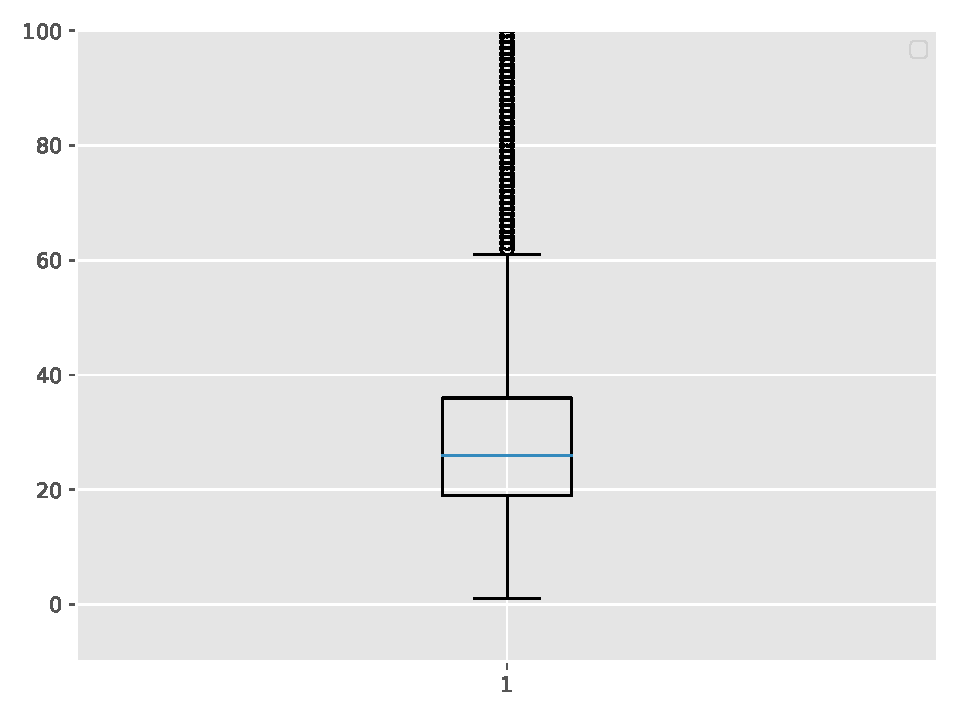
\includegraphics[width=0.75\linewidth]{images/analysis/histogram-lengths.pdf}
    \caption{Verteilung der Sequenzlängen im Datensatz }
    \label{fig:sequence-lengths}
\end{figure}

Ein Fehler in der Implementierung hat zu Beginn dazu geführt, dass für jeden Namen jeweils nur das letzte Zeichen bzw. die Stoppmarke trainiert wurde.
Interessanterweise hat selbst dieses Modell nach hinreichend langem Training zu einigen brauchbaren Ausgaben (aber hauptsächlich unlesbaren Zeichenfolgen) geführt.
Zum Vergleich mit den Ausgaben der korrekten Implementierung sind die Ausgaben des fehlerhaften Codes im Abschnitt «Resultate» (\ref{ch:results}) aufgelistet.

Bisher war das Modell so implementiert, dass jede Epoche jeweils die gleichen Trainingseinheiten erhielt.
Der Grund für dieses Vorgehen basierte auf der Annahme, dass jede Trainingseinheit mehrmals dem Modell vorgelegt werden müsse, damit der Lernprozess effektiv ist.
Diese Annahme entstand jedoch auf der fehlerhaften Implementierung, weshalb sie verworfen werden kann.

Der Nachteil war, dass das Modell eine relativ begrenztes Trainingsset zu sehen bekam.
Dieser Nachteil verstärkt sich, da durch das behobene und nun korrekt funktionierende Training noch weniger Trainingseinheiten verwendet werden.
Bei einer Median-Zeilenlänge von 26 Zeichen (siehe Abb. \ref{fig:sequence-lengths}) sowie 500 Mini-Batches à 100 Trainingsschritten werden dem Modell also:

\[ 500 \cdot \frac{100}{26} = 1'923.1 \]

gerade mal rund 1900 Zeilen der insgesamt 400'000 Zeilen gezeigt.
Damit erlernt das Modell ein sehr begrenztes Vokabular.
Die Trainingslogik soll nun so verbessert werden, dass jede Epoche einen beliebigen Ausschnitt aus allen Zeilen zum Training erhält.
Der Loader wird als Endlosgenerator implementiert.
Erreicht eine Epoche das Ende des Datensatzes, wird wieder von vorne begonnen.
Gleichwohl mit dem Datensatz, der zur Validierung herangezogen wird.
Der Generator wird also quasi als Ringspeicher implementiert wobei Trainings- und Validierungsdatensatz um die Hälfte der Länge des Gesamtdatensatzes
verschoben («Offset») ausgeliefert werden.
Damit der ganze Datensatz mindestens einmal durchlaufen wird müssten also insgesamt rund \[ 26 \cdot 422039 = 10'973'014 \] Trainingsschritte vollführt werden.
Wird von einer idealen Mini-Batch-Grösse von 100 Trainingsschritten ausgegangen, fallen insgesamt \[ \frac{109'730'14}{100} = 109'730 \] Mini-Batches an.
Damit kann die Anzahl der notwendigen Mini-Batches für einen bestimmten Prozentsatz des Gesamtdatensatzes als Funktion $ b(p, e) $ ausgedrückt werden:

\[ b(p, e) = \frac{p \cdot R \cdot S}{B \cdot e} \]

wobei $ p $ dem gewünschten Abdeckungsanteil des Datensatzes entspricht, $ e $ die Anzahl Epochen darstellt und die Konstanten $ R $, $ S $ sowie $ B $ die Anzahl Trainingssätze (Zeilen), die Median-Zeichenzahl pro Zeile sowie
die ideale Mini-Batch-Grösse repräsentieren.

Sollen also beispielsweise 25\% des gesamten Datensatzes mit 50 Epochen trainiert werden, so fallen:

\[ b(0.25, 50) = \frac{0.25 \cdot 422039 \cdot 26}{125 \cdot 50} = 438.92 \]

Mini-Batches pro an.
Diese Funktion dient dem Loader dazu, das Modell entsprechend lange zu trainieren.

\subsection{Hinzufügen eines Steuerparameters (Jahreszahl)}
\label{subsec:adding-time-component}

Jeder Trainingssatz bzw. jede Gerichtbezeichnung ist mit einem Datum versehen, an dem das Gericht zum ersten Mal
registriert wurde sowie mit einem Datum, an dem das Gericht zum letzen Mal registriert wurde.
Ein Histogram legt offen, dass die einzelnen Gerichte ungleichmässig auf die Zeit verteilt ist.
Ausserdem weist der Grossteil der Gerichte eine «Lebensdauer» von wenigen Jahren auf (siehe Abb.\ref{fig:hist-dates-datespans}).
Aufgrund letztgenannter Tatsache soll das Enddatum einfachheitshalber ignoriert werden.
Stattdessen wir das Eintrittsdatum der Eingabesequenz für das Modell angehängt.
Da nach erstem Ausprobieren das Anfügen der absoluten Jahreszahl kein gutes Training ermöglichte, wird das Jahr
als relativer Wert in einer Jahresspanne von 300 Jahren (1800 - 2100) angehängt, wobei also 0.0 dem Jahr 1800 sowie
der Wert 1.0 dem Jahr 2100 entsprechen.
Wurde zuvor das Zeichen «B» in Form eines One-Hot-Vektors $ (0.0, 0.0, 1.0, 0.0, 0.0)^{T} $ an das Modell übergeben,
so wird nun der Vektor um die Jahreszahl (z.B. 1975 = 0.583) erweitert zu $ (0.0, 0.0, 1.0, 0.0, 0.0, 0.583)^{T} $

\begin{figure}
    \centering
    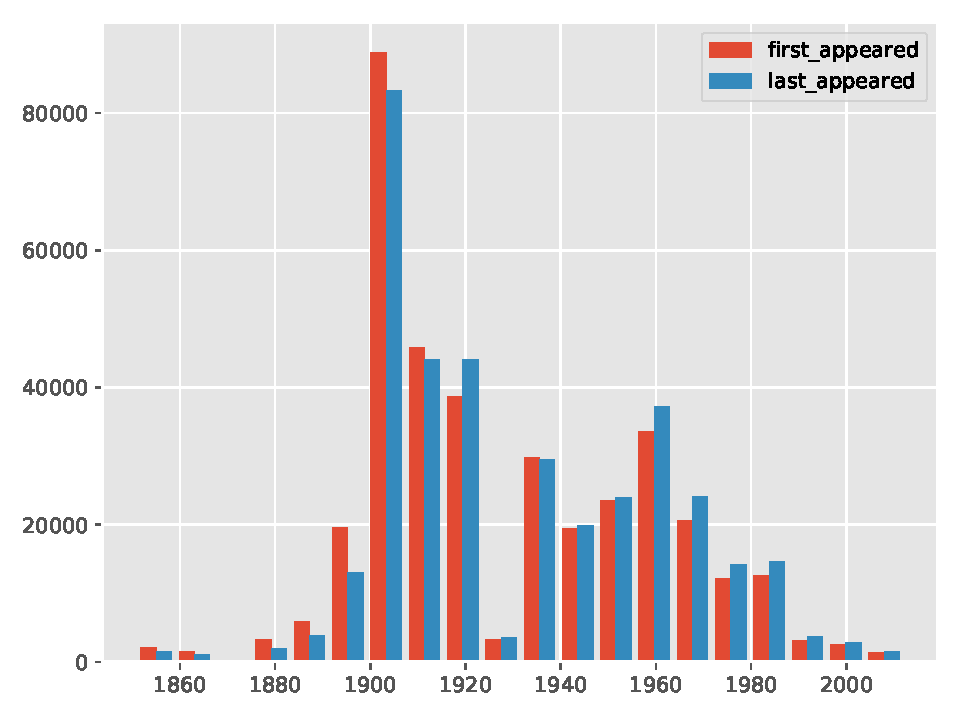
\includegraphics[width=0.75\linewidth]{images/analysis/histogram-dates.pdf}
    \caption{Zeitliche Verteilung}
    \label{fig:hist-dates-dates}
\end{figure}

\section{Erzeugung von Sequenzen}
\label{sec:model-generation}
    \chapter{Resultate}
\label{ch:results}

Dieser Abschnitt führt die durch das im vorherigen Abschnitt definierten Modell erzeugten Resultate auf und beschreibt sie.
Weil die Bewertung des Modells nur manuell und qualitativ möglich ist (d.h. Messwerte wie Präzision oder Recall korrelieren nicht zwingend
mit der wahrgenommenen Qualität der Ausgaben des Modells), ist es notwendig, dass die Ausgaben systematisch auf die verwendeten
Modellparameter zurückgeführt werden können.
Dafür wir das Modell systematisch mit unterschiedlichen Parametern trainiert, und die Resultate werden in einer
Konfigurationsmatrix aufgelistet.
Für jede Konfiguration werden die Initialsequenzen «A», «E», «I», «O», «U», «Chicken», «Steak», «Burger» und «Tomato» verwendet.
Für jede Konfiguration und jede Initialsequenz werden ausserdem jeweils drei Ausgaben erzeugt.

\begin{center}
    \begin{table}
        \centering
        \tiny
        \begin{tabular}{ |l|l|l| }

            \hline
            \textbf{} & \textbf{64 Units, val acc 49\%} & \textbf{512 Units, val acc 76\%} \\
            \hline
            \textbf{1 Layer} &
            \begin{tabular}[c]{@{}l@{}}

               Avota, Coffee, Season, Lobler, Nice Combinatiandi \\
               Ard Supremern Mambor Rolls (20 Omeley) (2 de \\
               Aspirale, Partreyning, Cocktamel, Handia Portion, Heas Ice B \\
               Eggs Holl: Coffee with Fresh Branches \\
               ERts with or Veal Holland Bour,, Butter, Salad Bowl with \\
               Extra Canfot Strawberringen Broiled Lamb Sandwich, Escelliny \\
               Isporit of Chicken \\
               Imported Sea Lemunish Limp Rib on Tarle \\
               Ice Cream, Beug \\
               Odes Potato  Rind Eocy-Fried Potatoes, Salad \\
               Oriex Coldoysh, Broth Bowl pinach) \\
               Orrerser Lobster and Butter, served with Chocolated Two Bord \\
               Undola New Chicken & Cream \\
               Utentelle Saude Craps or Peas, Coffee \\
               UVanori, Noodly Bosed with Chicken, Broiled Coffee, Rolls an \\
               Chicken and Breant \\
               Chicken Rib of Cream, Coffee Mad or Fresh Cane Yonktaa Blanch, Fre \\
               Chicken Peach Sinally Paddermi sauco \\
               Steak 25 Wenberner Dails, Beef Boiled Made Hollander with Fresh \\
               Steak cake and in with thriled smith, or Crablese, Cocktail (192 \\
               Steak, Lemon Madeluse STEAK VEGIT RYAMEL with French Fried Potat \\
               Burger with Salad and Spring Salad, sHELS SPRIMP AUL DABE \\
               Burger \\
               Burger (S.) Charent \\
               Tomato Butterrian Pie \\
               Tomato Coffee Sandwich, Pot Pork \\
               Tomato Tomato Tamered Sen Brothry Coffee, Fresh Fruits, Turlen,, \\

            \end{tabular} &
            \begin{tabular}[c]{@{}l@{}}

                Apricots, Layer Cake \\
                Arisotter's Sword Cheese, Tea and Dessert \\
                Aveck Made a OBARISION COCKTAIL (R.F.E. Regil) \\
                EWNEY COCKTAIE S9oth (Resart) \\
                Enchilada Cake \\
                English Mutton Chops, Ham, Puree Grilled in served with vinc \\
                Italian Decker \\
                Ice Cream, Parsley-Potato \\
                Italienne Lemon Horsicreme \\
                Oyster, Au Jus, French Dressing, Bread and Butter, Toast or \\
                Old English Cheese and Cream, Fresh Greens accia celery, win \\
                ORANGE Cockane \\
                Un Sirloin Steak, Dinner Stew \\
                UCYlet Bourbon Whisky \\
                Usher Cocktail \\
                Chicken Noodles, Dinner Salad \\
                Chicken Normoniscotod Beefsteak, Cookie Juice or Red Wine, Served \\
                Chicken a la Therking \\
                Steak, au Gratin Potatoes \\
                Steak a la Newburg \\
                Steak, French Fried Potatoes \\
                Burger Topps, Brandy, Fresh Mushrooms or Skresser, Cheddar Peau a \\
                Burger Scallops, Fried) \\
                Burgerstone-Crabmeat \\
                Tomato, Salad Bowl, Rolls, Coffee, Tea or Milk \\
                Tomato, Toast or Rolls, Beverage \\
                Tomato Surprise with Slices of Lettuce, Cole \\

            \end{tabular} \\
            \hline
            \textbf{5 Layers} & KZZkfvyyQexqTel & a bey \\
            \hline
        \end{tabular}
        \caption{Caption}
        \label{tab:first-sequences}
    \end{table}
\end{center}


\begin{center}
    \begin{table}
        \centering
        \begin{tabular}{ |l|l|l| }

            \hline
            \textbf{n} & \textbf{Initialsequenz} & \textbf{Generierte Sequenz} \\
            \hline
            1 & GVoRUcZybxnbknW & in Aones \\
            2 & KZZkfvyyQexqTel & a bey \\
            3 & oXvGKETlJftZHnE & SPhKAQahbgOCmjA \& pg. \\
            4 & TKWLvaUtsiBvjPm & Artonast wit Creme \\
            5 & fewKeuFYJecyCAk & Autt, cu paAte Sauce \\
            6 & ItekMqsKSONjbZj & gngn \\
            7 & KXntyJsfzrZFAJT & eatong \\
            8 & wudYekDhHOnsuPM & t \\
            9 & rOVMbLyCBbyCCSv & uAf \\
            10 & sGrYAEQfnkKxpOM & eiihg \\
            11 & jTNkWHsSswfEqhE & ing woth Mustorer) \\
            12 & bSTqiMSCZxVffMo & pshne Homatse \\
            13 & ktJyYYRuSUIJrCk & ung, D AyAnena aute,ors \\
            14 & kfoHrzlsoUGsAkY & Ah DricrTela oedt \\
            15 & DLVzoGsxmAwZgNZ & PoRrer \\
            16 & LCgtubworFrYewb & anco Hadorige \\
            17 & XchjpBUGSMyTMDq & ung \\
            19 & uNjcueOEZadlCMi & ihon w anilh Potatoast \\
            20 & UqStcroEvEehEyo & ng aust (torofffeds \\
            22 & ITiVXrEVDZXmROr & i, Are \& OoTatots \\
            23 & qweSAvVKPXrITCg & eagO \\
            26 & HfhoDhwJzEQaENT & \& Bance \\
            27 & XESvYRSRqVSVNQy & iAe, D' Arerel \& Sauce Potator \\
            28 & CswghmMaYkvPCbR & ete wite withe Bacons onito \\
            29 & tfRfupMQNvfAiaM & n Ar) \\
            30 & DdeFQkxYiMRYZdS & eupe \\
            31 & EcWjyUUvFZlzIVr & ieegs \\
            32 & seJxLpTqfwVrXap & jUTKKjCUByrALrS \& , Pon oof CTEes \\
            33 & jkAdzFdrlJDiQrI & ig anu Fueneons \\
            34 & ZItmxxUhqrlSXOI & b \\
            36 & ZhkCmYpZooVaFbs & e \\
            37 & jKbYNXXLpnbCgOd & Ait \\
            38 & wdaAgOuxYYhomCF & ith shune \\
            \hline
        \end{tabular}
        \caption{Caption}
        \label{tab:first-sequences}
    \end{table}
\end{center}

\begin{center}
    \begin{table}
        \centering
        \begin{tabular}{ |l|l|l| }

            \hline
            \textbf{n} & \textbf{Initialsequenz} & \textbf{Generierte Sequenz} \\
            \hline
            1 &  heyvAgaJnFEykXR & ROyooA SFac,a BaNooe \\
            2 &  qApRVwGkLZaRTpY & YoClNE AN COuuvE SARS \\
            3 &  hSSBSghZgvntYKW & WNOy \\
            4 &  FDtdLiovThWAABB & BaAsSA SALL IET CONDE, BRER AMBRA SUER, SIUTALIRA SLUERE BEE \\
            5 &  exvduWkBRXPNgNc & casOy BSTTESSaSTAS, Ay STENLLOWSFe \\
            6 &  pjJugwZkcVtIaHT & TEE AAa OpBu'E LAUj \\
            7 &  vYDTlKoBjHctHLM & Mer Em \\
            8 &  EATxlnekKSyyhXi & if Spakess \\
            9 &  VacBJsKUBwxBydg & gnodPHasdLirsh\& Salcok \\
            10 & DzEnFccEnDbgdHI & IEs \\
            11 & WVaBhFZTILSnQUj & jeTEEE \\
            12 & tuTluUGOpjxkryK & KraANdd Nedd \\
            13 & OKRABqePBWpocxI & Indeas \\
            14 & VzXKNFSsVfYfzlg & ge ois Ned M'llet \\
            15 & SuxVLdnvkkCacoq & qu \\
            16 & leIMviMndJaIjSb & bo org, BL OUG \\
            17 & LOFFoVRpWHMonHv & vA, TETLa \\
            19 & UkjuVIJtjoUpLIB & BTONCEETS \\
            20 & yWMmVISehLIBXoh & h \\
            22 & QHzgFhRXrsfwHnD & DhoAs,ucheredaldesri \\
            23 & sMhAWWJdrTjcjsN & Ned \\
            26 & GNGyQTKJgvxfPtK & KasagB \\
            27 & QPVDHuCtxfHrReF & F Su Sak OIp,, Ay oes Oes \\
            28 & czXXfUdrbYuxQaw & was \\
            29 & WigGaQAfkvSgyAV & Ve, LOIroua Aw CerE's \\
            30 & TfgDYRHCSXRnjDv & vELLEILLINTITEK,IS, ROUDOUYA \\
            31 & vwrTcebqyXvKChl & ls, crowmerrbous e \\
            32 & WpjVUIxzQbHbRoJ & J TEUE \\
            33 & bjXkBNwONnuriUT & TEF YEE \\
            34 & SUwXNVDHGuyrPXZ & ZANE,II  O N Ay CREp \\

            \hline
        \end{tabular}
        \caption{Caption}
        \label{tab:first-sequences-after-fix}
    \end{table}
\end{center}


\begin{center}
    \begin{table}
        \centering
        \resizebox{\textwidth}{!}{
        \begin{tabular}{ |l|l|l|l|l| }

            \hline
            \textbf{n} & \textbf{Initialsequenz} & \textbf{Generierte Sequenz 64} & \textbf{Generierte Sequenz 256} & \textbf{Generierte Sequenz 512} \\
            \hline
            1 & GVoRUcZybxnbknW & Whea & WUag Dalen & WhipTer ba ch pind Camb eits \\
            2 & TKWLvaUtsiBvjPm & moshrin  Musr rumst wchet & me & mon tarte\\
            3 & fewKeuFYJecyCAk & kfand & kglanY acol & knssaraw andderes \\
            4 & KXntyJsfzrZFAJT & T & T muthe & Te \\
            5 & jTNkWHsSswfEqhE & E, CoN Oy Lp My DfOTBRENOa  F TOINO & Eg S \& CE BLUUCR\& OTREAS, SAUL Yo Sauc & Et \& E sansere, Soulles \\
            6 & uNjcueOEZadlCMi & i, Aal are & in, & ingere \\
            7 & XESvYRSRqVSVNQy & yE, DAy NANG Lea DO CEg OAE & yUN Ef BUN SAMCE & yETT MAATEEAl \\
            8 & EcWjyUUvFZlzIVr & rF FAy Busdee B YoNNed Friodd & r ongKice & riss wAth cre \\
            9 & A & Apples & Apples & Apples \\
            10 & B & Baked apples with cream & Baked apples with cream & Baked apples with cream \\
            11 & C & Chicken broth & Chicken broth & Chicken broth \\
            12 & Chicken & n broth & n broth & n broth \\
            \hline
        \end{tabular}
        }
        \caption{Fixierte Initialsequenzen zur Untersuchung verschiedener Modellkonfigurationen}
        \label{tab:fixed-initial-sequences1}
    \end{table}

\end{center}

\begin{center}
    \begin{table}
        \centering
        \resizebox{\textwidth}{!}{
        \begin{tabular}{ |l|l|l|l|l| }

            \hline
            \textbf{n} & \textbf{Initialsequenz} & \textbf{Generierte Sequenz 64, L1, D0.1} & \textbf{Generierte Sequenz 62, L3, D0.1} & \textbf{Generierte Sequenz 64, L5 D0.1} \\
            \hline
            1 & GVoRUcZybxnbknW & in Aones & WSrh' chhompagntsos tret & Whreast \\
            2 & TKWLvaUtsiBvjPm & Artonast wit Creme & mERNT Dooo D GEN, M.lerr LNNe, Po.us PTENBe Nock FuNer rifd & mels \\
            3 & fewKeuFYJecyCAk & Autt, cu paAte Sauce & kripl & ky Snonle \\
            4 & KXntyJsfzrZFAJT & eatong & Toratt & Tinse \\
            5 & jTNkWHsSswfEqhE & ing woth Mustorer) & Es & Erg \\
            6 & uNjcueOEZadlCMi & ihon w anilh Potatoast & ih & inds \\
            7 & XESvYRSRqVSVNQy & iAe, D' Arerel \& Sauce Potator & y BRoNffrotd & yK \\
            8 & EcWjyUUvFZlzIVr & ieegs & r \& OfxTEe s & rer \\
            9 & A & kee & Apples & Apples \\
            10 & B & amb & Boiled onions, cream sauce & Baked apples with cream \\
            11 & C & \&. & \& Chicken broth & Chicken broth \\
            12 & Chicken & & n broth & n broth \\
            \hline
        \end{tabular}
        }
        \caption{Fixierte Initialsequenzen zur Untersuchung verschiedener Modellkonfigurationen}
        \label{tab:fixed-initial-sequences2}
    \end{table}

\end{center}

\begin{center}
    \begin{table}
        \centering
        \resizebox{\textwidth}{!}{
        \begin{tabular}{ |l|l|l|l|l| }

            \hline
            \textbf{n} & \textbf{Initialsequenz} & \textbf{Generierte Sequenz 64, 5000} & \textbf{Generierte Sequenz 64, 50000} & \textbf{Generierte Sequenz 64, 500000} \\
            \hline
            1 & GVoRUcZybxnbknW & in Aones & anteG in Cream & Whished Sureere \\
            2 & TKWLvaUtsiBvjPm & Artonast wit Creme & e with Milk with Bacon with Milk with Bacon with Milk with & mo\\
            3 & fewKeuFYJecyCAk & Autt, cu paAte Sauce & es) & ke \\
            4 & KXntyJsfzrZFAJT & eatong & ss & TZN CUSCACOUP PIT OY ALET Brackleass) 1/2 pot \\
            5 & jTNkWHsSswfEqhE & ing woth Mustorer) & vil)-aux champagonago & E. \\
            6 & uNjcueOEZadlCMi & ihon w anilh Potatoast & le Style & itte \\
            7 & XESvYRSRqVSVNQy & iAe, D' Arerel \& Sauce Potator & en Pee Sleate & yON \\
            8 & EcWjyUUvFZlzIVr & ieegs & eatlaine & avery & r \\
            9 & A & kee & \& & Assorted Cakes \\
            10 & B & amb & oxe & Broiled Spring Chicken Saute au gratin \\
            11 & C & \&. & rams & Cold Cocktails \\
            12 & Chicken & & & n Croquettes, Cream sauce \\
            \hline
        \end{tabular}
        }
        \caption{Fixierte Initialsequenzen zur Untersuchung verschiedener Modellkonfigurationen}
        \label{tab:fixed-initial-sequences}
    \end{table}

\end{center}

\begin{center}
    \begin{table}
        \centering
        \resizebox{\textwidth}{!}{
        \begin{tabular}{ |l|l|l|l|l| }

            \hline
            \textbf{n} & \textbf{Initialsequenz} & \textbf{Generierte Sequenz 64, 5000} & \textbf{Generierte Sequenz 256, 50000} & \textbf{Generierte Sequenz 64, 500000} \\
            \hline
            1 & GVoRUcZybxnbknW & in Aones & Wey & Whished Sureere \\
            2 & TKWLvaUtsiBvjPm & Artonast wit Creme & min & mo\\
            3 & fewKeuFYJecyCAk & Autt, cu paAte Sauce & ken Black, or Cotz, Gin & ke \\
            4 & KXntyJsfzrZFAJT & eatong & Tram Punch & TZN CUSCACOUP PIT OY ALET Brackleass) 1/2 pot \\
            5 & jTNkWHsSswfEqhE & ing woth Mustorer) & Ex& E. \\
            6 & uNjcueOEZadlCMi & ihon w anilh Potatoast & irontan, Pine Sauce & itte \\
            7 & XESvYRSRqVSVNQy & iAe, D' Arerel \& Sauce Potator & y & yON \\
            8 & EcWjyUUvFZlzIVr & ieegs & eatlaine & rI & r \\
            9 & A & kee & Anchovies & Assorted Cakes \\
            10 & B & amb & Bluefish & Broiled Spring Chicken Saute au gratin \\
            11 & C & \&. & Calf's head, fried with tomato sauce & Cold Cocktails \\
            12 & Chicken & & n croquette, with peas & n Croquettes, Cream sauce \\
            \hline
        \end{tabular}
        }
        \caption{Fixierte Initialsequenzen zur Untersuchung verschiedener Modellkonfigurationen}
        \label{tab:fixed-initial-sequences}
    \end{table}

\end{center}


\begin{figure}
    \centering
    \includegraphics[width=0.75\linewidth]{}
    \caption{Fehler in der Logik: Statt der gesamten Abfolge wird jeweils nur der letzte Buchstabe trainiert.}
    \label{fig:logic-error}
\end{figure}

512
47s 9ms/step - loss: 0.0272 - accuracy: 0.9799 - val_loss: 4.9989 - val_accuracy: 0.3500

50000
Epoch 00001: val_accuracy improved from -inf to 0.45450, saving model to checkpoints/checkpoint_100_500_50_64_1_0_15.best_val_acc.hdf5


Weiterentwicklung:

System, wo Benutzer Vorschläge bewerten kann -> Einspeisung in netz
    \chapter{Auswertung \& Ausblick}
\label{ch:analysis}

\subsection{Erhöhung der LSTM-Einheiten}
\label{subsec:increase-lstm}

\subsection{Erhöhung der LSTM-Schichten}
\label{subsec:increase-lstm-layers}

\subsection{Erhöhung der Trainingsdatensätze}
\label{subsec:increase-num-dataset}

\subsection{Erhöhen der Zufälligkeit}
\label{subsec:increase-randomness}

So wie in \autocite{dabbura} soll der nächste Buchstabe zufällig ausgewählt werden
https://docs.scipy.org/doc/numpy/reference/generated/numpy.random.choice.html

    \chapter*{Glossar}
\addcontentsline{toc}{chapter}{Glossar}
\renewcommand{\glossarysection}[2][]{}

\printglossaries





    \printbibliography[<options for printing>]

    \listoffigures


\end{document}
